\documentclass[11pt,oneside]{article}	%use"amsart"insteadof"article"forAMSLaTeXformat
\usepackage{geometry}		%Seegeometry.pdftolearnthelayoutoptions.Therearelots.
\geometry{letterpaper}		%...ora4paperora5paperor...
%\geometry{landscape}		%Activateforforrotatedpagegeometry
%\usepackage[parfill]{parskip}		%Activatetobeginparagraphswithanemptylineratherthananindent
\usepackage{graphicx}				%Usepdf,png,jpg,orepsßwithpdflatex;useepsinDVImode
								%TeXwillautomaticallyconverteps-->pdfinpdflatex		
\usepackage{amssymb}
\usepackage{hyperref}

%----macros begin-----------------------------------------------------------------------------------
\usepackage{graphicx}
\usepackage{color}
\usepackage{amsthm}

%\renewenvironment{Shaded}{\pause\begin{snugshade}}{\end{snugshade}}
\def\twocolumns#1#2{\begin{columns}
\begin{column}{0.5\linewidth}#1\end{column}
\begin{column}{0.5\linewidth}#2\end{column}
\end{columns}}
\def\mytwocolumns#1#2#3#4{\begin{columns}
\begin{column}{#1\linewidth}#2\end{column}
\begin{column}{#3\linewidth}#4\end{column}
\end{columns}}
\def\mythreecolumns#1#2#3#4#5#6{\begin{columns}
\begin{column}{#1\linewidth}#2\end{column}
\begin{column}{#3\linewidth}#4\end{column}
\begin{column}{#5\linewidth}#6\end{column}
\end{columns}}
\def\threecolumns#1#2#3{\begin{columns}
\begin{column}{0.33\linewidth}#1\end{column}
\begin{column}{0.33\linewidth}#2\end{column}
\begin{column}{0.33\linewidth}#3\end{column}
\end{columns}}
\def\fourcolumns#1#2#3#4{\begin{columns}%
\begin{column}{0.25\linewidth}#1\end{column}%
\begin{column}{0.25\linewidth}#2\end{column}%
\begin{column}{0.25\linewidth}#3\end{column}%
\begin{column}{0.25\linewidth}#4\end{column}%
\end{columns}}

\def\conv{\mbox{\textrm{conv}\,}}
\def\aff{\mbox{\textrm{aff}\,}}
\def\E{\mathbb{E}}
\def\R{\mathbb{R}}
\def\Z{\mathbb{Z}}
\def\tex{\TeX}
\def\latex{\LaTeX}
\def\v#1{{\bf #1}}
\def\p#1{{\bf #1}}
\def\T#1{{\bf #1}}

\def\vet#1{{\left(\begin{array}{cccccccccccccccccccc}#1\end{array}\right)}}
\def\mat#1{{\left(\begin{array}{cccccccccccccccccccc}#1\end{array}\right)}}

\def\lin{\mbox{\rm lin}\,}
\def\aff{\mbox{\rm aff}\,}
\def\pos{\mbox{\rm pos}\,}
\def\cone{\mbox{\rm cone}\,}
\def\conv{\mbox{\rm conv}\,}
\newcommand{\homog}[0]{\mbox{\rm homog}\,}
\newcommand{\relint}[0]{\mbox{\rm relint}\,}

%----macros end-----------------------------------------------------------------------------------


\title{Testing Literate Programming}
\author{TheAuthor}
%\date{}							%Activatetodisplayagivendateornodate

\begin{document}
\maketitle
\nonstopmode


\begin{abstract}
This document is my first effort on writing some literate programming~\cite{Knuth:1984:LP:473.479,Knuth:1992:LP:129057}, aiming to provide the best embedded documentation for my experimental code, while developing it. The tool choosen is \emph{nuweb}, in my view the simplest multi-language derivation from the Knuth's original WEB and CWEB tools~\cite{Knuth:1994:CSS:561208}. My approach to literate programming is also motivated by the wish for independency of the content from a specific programming language. Actually, I have several candidate languages --- including \texttt{python}, \texttt{haskell}, and \texttt{clojure} --- to use for writing the reference documentation for my research work, so that \emph{nuweb} gives me the freedom to freely experiment with them, even mixing chunks of code written in different languages in the same document, while providing an execution environment and unit testing in the same time. 
\end{abstract}

\tableofcontents
\newpage

\section{Introduction}

The  intent of this document is writing the reference documentation for an experimental algorithm aiming at generating the \emph{signed} incidence coefficients of the boundary and coboundary matrices for a complex of convex cells generated and handled using the LAR representation scheme recently developed by Vadim Shapiro, Antonio DiCarlo and me.

The main idea of this algorithmic approach is to use a geometric realisation of the cell complex as a simplicial complex, by extending the orientations of cells and the relative signed incidence coefficients from simplices to polytopes, so providing a robust, but yet simple way to compute the operator matrices in the realm of general convex cells.

\subsection{Preview}
In Section~\ref{simplicial} we discuss how to generate a simplicial complex and how to compute its (co)boundary operator matrices. In Section~\ref{cuboidal} we generate a $T$-complex of cuboidal cells, and we extract its skeleton complexes of dimension 2 and 1. In Section~\ref{polytopal} we finally approach the problem of generating a (co)boundary matrix with signed coefficients, and fully implement an algorithm for its generation in the general case.



\section{Signed (co)boundary matrices of a simplicial complex}
\label{simplicial}

\paragraph{Importing the library}
First of all, a modeling application having to deal with simplicial complexes must import the $Simple_X^n$ library, denoted \texttt{smplxn} in \texttt{python}. The name of the library was firstly used by our CAD Lab at University of Rome ``La Sapienza'' in years 1987/88 when we started working with dimension-independent simplicial complexes~\cite{Paoluzzi:1993:DMS:169728.169719}. This one in turn imports some functions from the \texttt{scipy} package and the geometric library \texttt{pyplasm}~\cite{}.

%-------------------------------------------------------------------------------
@d Inport the $Simple_X^n$ library
@{import sys
sys.path.insert(0, 'lib/py/')
from smplxn import *
@}
%-------------------------------------------------------------------------------

\subsection{Structured grid}

\subsubsection{2D example}

\paragraph{Generate a simplicial decomposition}
Then we generate and show a 2D decomposition of the unit square $[0,1]^2\subset\E^2$ into a $3\times 3$ grid of simplices (triangles, in this case), using the \texttt{simplexGrid} function, that returns a pair \texttt{(V,FV)}, made by the array \texttt{V} of vertices, and by the array \texttt{FV} of ``faces by vertex'' indices, that constitute a \emph{reduced} simplicial LAR of the $[0,1]^2$ domain. The computed \texttt{FV} array is then dispayed ``exploded'', being $ex,ey,ez$ the explosion parameters in the $x,y,z$ coordinate directions, respectively. Notice that the \texttt{MKPOLS} pyplasm primitive requires a pair \texttt{(V,FV)}, that we call a ``model'', as input --- i.e. a pair made by the array \texttt{V} of vertices, and by a zero-based array of array of indices of vertices. Elsewhere in this document we identified such a data structure as CSR$(M_d)$, for some dimension $d$. Suc notation stands for the Compressed Sparse Row representation of a binary characteristic matrix.

%-------------------------------------------------------------------------------
@d Generate a simplicial decomposition ot the $[0,1]^2$ domain
@{V,FV = simplexGrid([3,3])
VIEW(EXPLODE(1.5,1.5,1.5)(MKPOLS((V,FV))))
@}
%-------------------------------------------------------------------------------

\paragraph{Extract the $(d-1)$-faces}
Since the complex is simplicial, we can directly extract its facets (in this case the 1-faces, i.e. its edges) by invoking the \texttt{simplexFacets} function on the argument \texttt{FV}, so returning the array \texttt{EV} of ``edges by vertex'' indices. 

%-------------------------------------------------------------------------------
@d Extract the edges of the 2D decomposition
@{EV = simplexFacets(FV)
ex,ey,ez = 1.5,1.5,1.5
VIEW(EXPLODE(ex,ey,ez)(MKPOLS((V,EV))))
@}
%-------------------------------------------------------------------------------

\paragraph{Export the executable file}
We are finally able to generate and output a complete test file, including the visualization expressions. This file can be executed by the \texttt{test} target of the \texttt{make} command.

%-------------------------------------------------------------------------------
@O test/py/test01.py
@{
@<Inport the $Simple_X^n$ library@>
@<Generate a simplicial decomposition ot the $[0,1]^2$ domain@>
@<Extract the edges of the 2D decomposition@>
@}
%-------------------------------------------------------------------------------

\subsubsection{3D example}

In this case we produce a $2\times 2\times 2$ grid of tetrahedra. The dimension (3D) of the model to be generated is inferred by the presence of 3 parameters in the parameter list of the \texttt{simplexGrid} function. 

%-------------------------------------------------------------------------------
@d Generate a simplicial decomposition ot the $[0,1]^3$ domain
@{V,CV = simplexGrid([2,2,2])
VIEW(EXPLODE(1.5,1.5,1.5)(MKPOLS((V,CV))))
@}
%-------------------------------------------------------------------------------

and repeat two times the facet extraction:

%-------------------------------------------------------------------------------
@d Extract the faces and edges of the 3D decomposition
@{
FV = simplexFacets(CV)
VIEW(EXPLODE(1.5,1.5,1.5)(MKPOLS((V,FV))))
EV = simplexFacets(FV)
VIEW(EXPLODE(1.5,1.5,1.5)(MKPOLS((V,EV))))
@}
%-------------------------------------------------------------------------------

and finally export a new test file:

%-------------------------------------------------------------------------------
@O test/py/test02.py 
@{
@<Inport the $Simple_X^n$ library@>
@<Generate a simplicial decomposition ot the $[0,1]^3$ domain@>
@<Extract the faces and edges of the 3D decomposition@>
@}
%-------------------------------------------------------------------------------


\subsection{Unstructured grid}


\subsubsection{2D example}


\subsubsection{3D example}




\section{Generation of LAR of a cuboidal complex}
\label{cuboidal}

\section{Algorithm for signed (co)boundary of a polytopal complex}
\label{polytopal}

A top-down view of the program structure is as follows:

%-------------------------------------------------------------------------------
@O test/py/test06.py
@{
@<Inport the $Simple_X^n$ library@>
@<Vertex array@>
@<3D-cells CSR matrix@>
@<2D-face CSR matrix@>
@<1D-edge CSR matrix@>
@<main@>
@}
%-------------------------------------------------------------------------------

\[
\alpha, A, \beta, B, \gamma, \Gamma, \pi, \Pi, \phi, \varphi, \Phi
\]

%-------------------------------------------------------------------------------
@d Vertex array
@{
V = [[4,10,0.0*2], [4,10,1.0*2], [4,10,2.0*2], [8,10,0.0*2], [8,10,1.0*2], [8,10,
2.0*2], [14,10,0.0*2], [14,10,1.0*2], [14,10,2.0*2], [8,7,0.0*2], [8,7,1.0*2], 
[8,7,2.0*2], [14,7,0.0*2], [14,7,1.0*2], [14,7,2.0*2], [4,4,0.0*2], [4,4,1.0*2], 
[4,4,2.0*2], [8,4,0.0*2], [8,4,1.0*2], [8,4,2.0*2], [14,4,0.0*2], [14,4,1.0*2], 
[14,4,2.0*2]] 
@|  V @}
%-------------------------------------------------------------------------------

%-------------------------------------------------------------------------------
@d 3D-cells CSR matrix
@{
CV = [[0,1,3,4,9,10,15,16,18,19],[1,2,4,5,10,11,16,17,19,20],[3,4,6,7,9,10,12,13
],[4,5,7,8,10,11,13,14],[9,10,12,13,18,19,21,22],[10,11,13,14,19,20,22,23]]
@|  CV @}
%-------------------------------------------------------------------------------


%-------------------------------------------------------------------------------
@d 2D-face CSR matrix
@{
FV = [[0,3,9,15,18],[1,4,10,16,19],[2,5,11,17,20],[3,6,9,12],[4,7,10,13],[5,8,
11,14],[9,12,18,21],[10,13,19,22],[11,14,20,23],[0,1,3,4],[0,1,15,16],[1,2,4,5],
[1,2,16,17],[3,4,6,7],[3,4,9,10],[4,5,7,8],[4,5,10,11],[6,7,12,13],[7,8,13,14],
[9,10,12,13],[9,10,18,19],[10,11,13,14],[10,11,19,20],[12,13,21,22],[13,14,22,23
],[15,16,18,19],[16,17,19,20],[18,19,21,22],[19,20,22,23]]
@|  FV @}
%-------------------------------------------------------------------------------

%-------------------------------------------------------------------------------
@d 1D-edge CSR matrix
@{
EV = [[0,3],[0,15],[1,4],[1,16],[2,5],[2,17],[3,6],[3,9],[4,7],[4,10],[5,8],[5,
11],[6,12],[7,13],[8,14],[9,12],[9,18],[10,13],[10,19],[11,14],[11,20],[12,21],
[13,22],[14,23],[15,18],[16,19],[17,20],[18,21],[19,22],[20,23],[0,1],[1,2],[3,
4],[4,5],[6,7],[7,8],[9,10],[10,11],[12,13],[13,14],[15,16],[16,17],[18,19],[19,
20],[21,22],[22,23]]
@|  EV @}
%-------------------------------------------------------------------------------


%-------------------------------------------------------------------------------
@d main
@{
simplices = pivotSimplices(V,CV,d=3)

VIEW(STRUCT([
			MKPOL([V,AA(AA(lambda k : k+1))(simplices),[]]),
			STRUCT(MKPOLS((V,EV)))
			]))

print"\nsimplexOrientations(simplices) =", simplexOrientations(V,simplices),"\n"
@|  simplices pivotSimplices @}
%-------------------------------------------------------------------------------


\begin{figure}[htbp] %  figure placement: here, top, bottom, or page
   \centering
   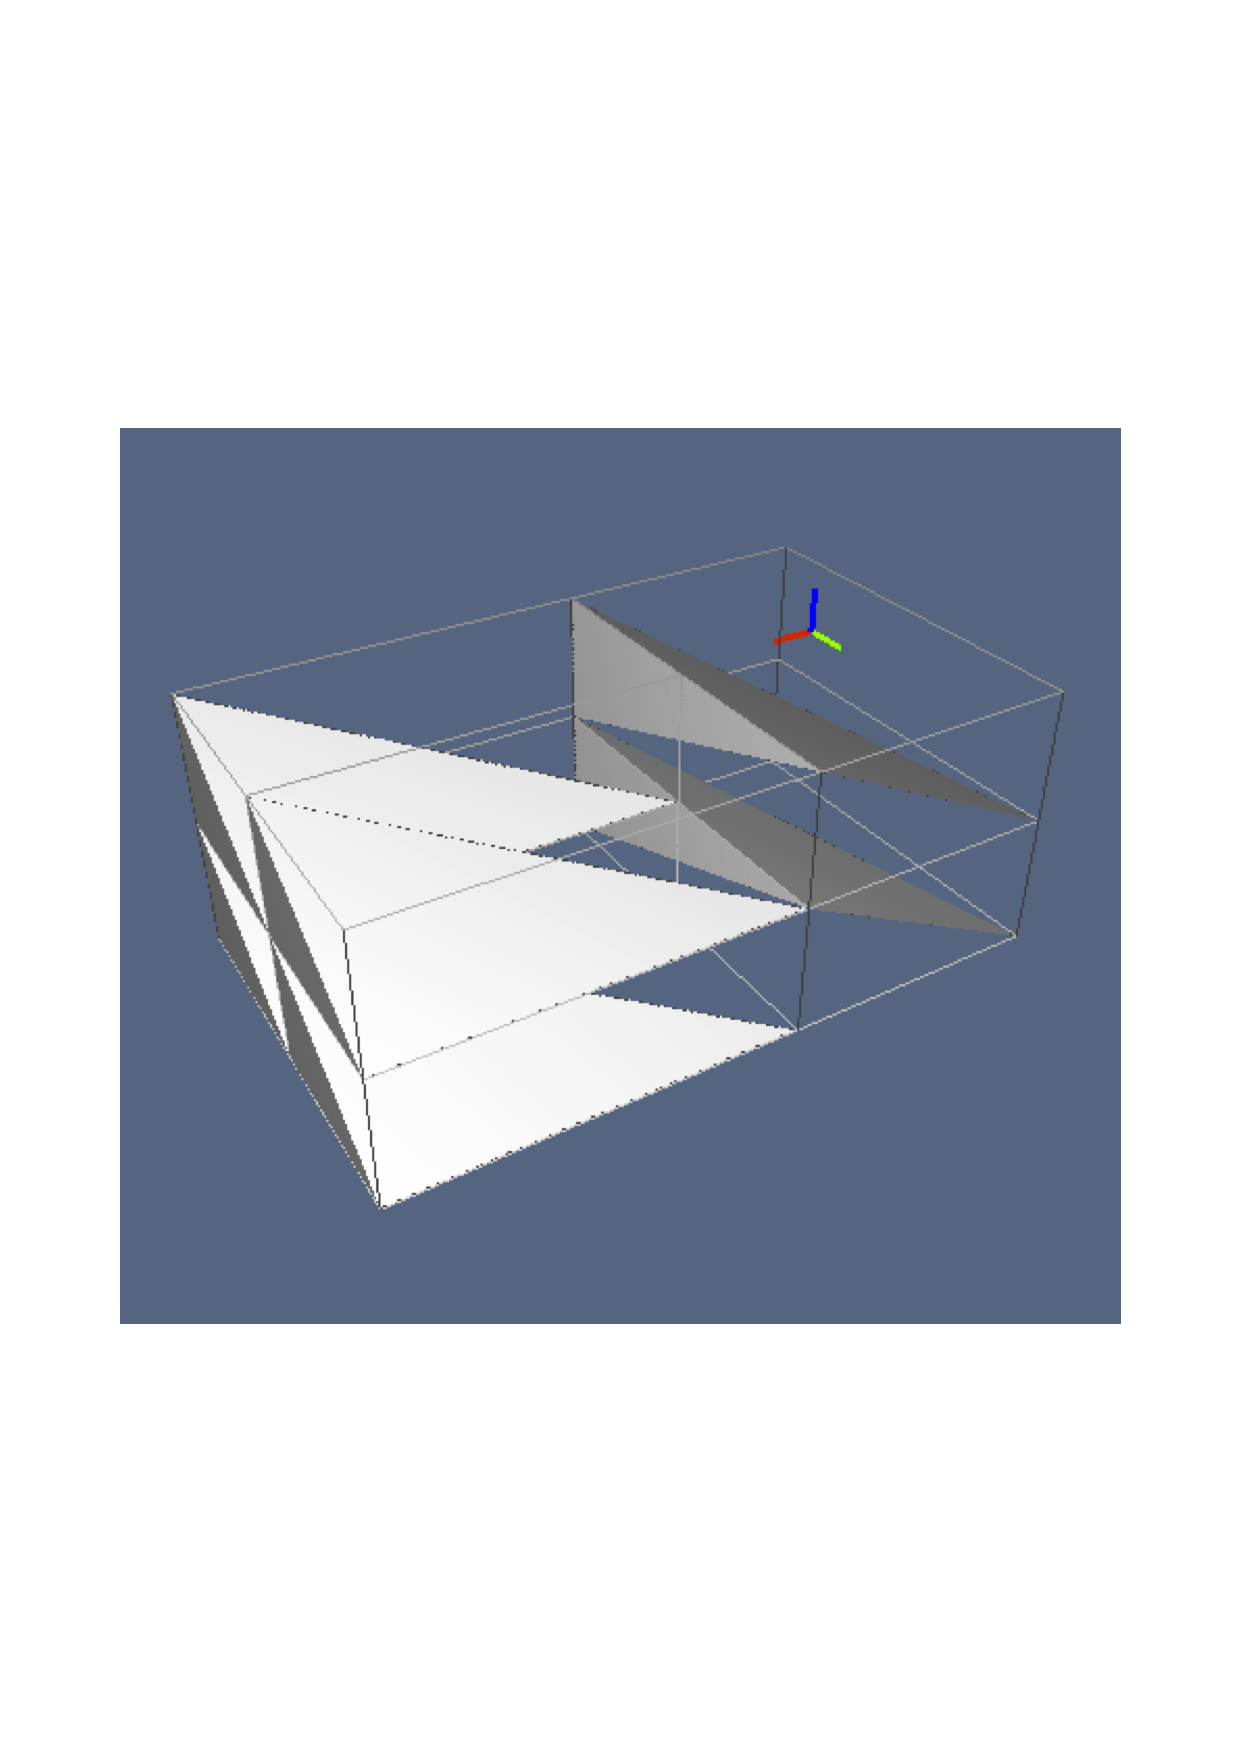
\includegraphics[width=0.6\linewidth]{images/fig1} 
   \caption{example caption}
   \label{fig:example}
\end{figure}

\section{Index}
\subsection*{Index of variables}
@u

\subsection*{Index of macros}
@m


\bibliographystyle{amsalpha}
\bibliography{cclar.bib}
        
\appendix
\end{document}